\section{Data and metadata sources}\label{data_sources}
\subsection{Observations}
\subsubsection{The International Comprehensive Ocean-Atmosphere Data Set}
% Background to marine met and coordination
Weather observations have routinely been made at sea since at least the 1650s, with descriptive observations of the prevailing weather conditions and early instrumental measurements included in the general ships logbooks as part of the daily entries. 
Following the Brussels Conference of 1853, and recognition of the importance of the weather observations to international trade and safe navigation, standardised meteorological logbooks and observing instructions were developed and made available to ships captains.
In return for following the instructions and returning the completed logbooks the captains were provided with the latest sailing directions and weather charts, thereby collectively gaining benefit from the collecting and sharing of meteorological data.
This international coordination, standardisation and data sharing has continued to the present day, currently overseen by the World Meteorological Organisation (WMO) and Global Ocean Observing System (GOOS) (e.g. see \cite{Smith2019}). Observations from other platforms, such as moored and drifting buoys, are similarly coordinated internationally.

% the global archives
Through the international coordination and data sharing, national weather services independently developed global archives of marine meteorological and oceanographic observations.
Many of these archives contained overlapping data. 
For example, the US Navy Marine Atlases developed after the Second World War contained data from both the US archives and data from, inter alia, the UK, German and Netherlands archives that had been shared internationally. 
This resulted in increased numbers of observations but at the expense of having to perform duplicate detection and elimination.
In recognition of the importance of historic data to understanding climate variability, building on the earlier Marine Atlases, the US National Oceanic and Atmospheric Administration (NOAA) developed the Comprehensive Ocean - Atmosphere Data Set (COADS) in the early 1980s.
The first version was published in 1985 (e.g. see \cite{Woodruff1987}), consisting of both monthly summary statistics for selected ECVs and the raw weather reports from ships and other vessels used as input to the monthly summaries.
Each weather report contained coincident measurements of multiple ECVs (typically air temperature and humidity, wind speed and direction, sea level pressure and sea surface temperature) together with visual estimates of the sea state, wind force (when not measured), cloud cover and weather. 
This first version formed the largest and most comprehensive archive of marine meteorological observations publicly available at the time. 

% where we are now, release 3.
Building on the first version, COADS continued to be developed with coverage extended to present day through major updates and reprocessing and through incremental near real time updates. 
As part of this development, and the evolving observing system, COADS has expanded from primarily ship based observations to surface meteorological measurements from most marine platforms shared internationally.
Examples include measurements from moored and drifting buoys, coastal stations and offshore platforms, all shared internationally in real time over the WMO Global Telecommunication System (GTS) and in delayed mode through Global Data Assembly Centres.
The development has also included blending COADS with other national archives and delayed mode data sources, such as the UK Met Office marine data bank.
In recognition of the importance of the international contributions COADS was renamed as the International Comprehensive Ocean - Atmosphere Data Set (ICOADS) in 2002 (e.g. \cite{Worley2005}). 
The current major release of ICOADS, release 3.0, was published in 2017 (\cite{Freeman2017}), releasing observations up to the end of 2014.
Near realtime updates for the period after 2014 are available from ICOADS Release 3.0.2 (\cite{Liu2022}).
The ICOADS near realtime updates contain regular releases of marine observations, updated within the first 10 days of the most current month. The near realtime observations are based on blended marine observations in the TAC and BUFR formats from NOAA's National Centers for Environmental Information (NCEI) GTS collections. 

% processing applied by ICOADS
As noted above, due to the combination of different sources over many decades, including from different national archives, and the long tradition of data sharing in marine meteorology there are many duplicates in the raw data. 
The publicly released version of ICOADS has attempted to remove or combine duplicates when detected, but this has not always been optimal due to choices made over the history of ICOADS. 
For example, some duplicates are missed due to one archive recording the latitude / longitude in whole degrees and another archive storing the same location information but recording the grid box centres (i.e. with a 0.5° trailing digit). 
These decisions have been revisited as part of this service, with the available ICOADS source files (known as "total" files within the NCEI/ICOADS archives) reprocessed and the data flagged appropriately.
This processing is described in Section \ref{processing}.
The original source of the data is recorded in ICOADS with the data accessions indexed by "deck" (DCK) and "source" (SID) identifiers (\cite{Woodruff1987}, \cite{Freeman2017}). 
A detailed summary of the data accessions is given in the marine inventory (C3S2\_D311\_Lot1.2.3.1\_202208\_Marine\_Inventory\_v2) (-TO BE UPDATED-) available from the CDS website.

\subsection{Selection of data for inclusion in Service}
As part of the development of this service the input sources and decks contributing observations to ICOADS have been prioritised and reprocessed based on the volume of observations, spatial / temporal coverage and availability of ECVs.

Release 1 focussed on the post World War II period (1951 - 2010) and included observations from drifting buoys (sea surface temperature and sea level pressure) and Voluntary Observing Ships (VOS) (air temperature, dew point temperature, wind speed and direction, sea level pressure and sea surface temperature).
As part of the first release VOS observations were merged with instrumental metadata from WMO Publication Number 47 (e.g.\cite{Kent2007}) to provide information on observing heights, instrument types / observing methods and information on the vessels contributing the observations. 

Release 2 sought to extend the record backwards to 1851, including all available ship observations prior to 1951.

Release 3 updated the record to the end of 2014. 

Release 4 updated the record to the end of 2020 using the observations from ICOADS Release 3.0.1, including a full reprocessing of the data from the previous releases. As part of this reprocessing additional metadata has been recovered for some of the earlier records and the observations for the period.

Release 5 updated the record to the end of 2021 using the observations from ICOADS Release 3.0.2, adding near realtime data updates including decoded BUFR messages from 2015 onwards.

Release 6, the most recent at the time, updated the record to the end of 2022 using the observations from ICOADS Release 3.0.2, migrated the data processing to the Irish Center for High-end Computing and fixed a bug where the additional metadata was not added in the past. The metadata has been added to the previous releases as a post-processing step.

Drifting buoy data from the ICOADS Release 3.0.2 are not included in this release.
A consolidated drifting buoy data record based on additional data sources such as the C-RAID Drifting buoys (\cite{craid}) will be processed and included in future releases.

The marine inventory (C3S2\_D311\_Lot1.2.3.1\_202208\_Marine\_Inventory\_v2, available from the CDS website) gives a detailed overview of the contents from each data source used in this release.

Figure \ref{fig:nreports-ts} shows the monthly number of reports available in the current release. 
Only those passing the full quality control check are shown, in total 390,335,546 reports from 248 sources have been processed.
Of these 282,367,426 are unique and pass the report quality control checks (see Section \ref{processing}), the remainder either fail the duplicate check or the aggregate report level QC check (see Section \ref{aggregate_qc}).
Figure \ref{fig:nreports-map} shows the spatial sampling by total number of reports and by number of months. 
The total number of reports is dominated by the recent decades and the increase in buoy sampling (see Figure \ref{fig:nreports-hovmoller}). 
The contribution to the ship based reports can be seen in the number of months available, with the ship tracks clearly visible.

Several notable sources and platform types have been excluded.
Namely, fixed stations (mobile installations and rigs, coastal stations and moored buoys), meteorological observations from research vessels, and meteorological observations from oceanographic programmes and datasets such as the World Ocean Database (WOD) and the Global Ocean Surface Underway Data (GOSUD). 
Users requiring access to these data are recommended to access data directly from the respective datasets (e.g. \href{https://www.ncei.noaa.gov/access/world-ocean-database-select/dbsearch.html} WOD, \href{http://www.gosud.org/}{GOSUD}, \href{https://samos.coaps.fsu.edu/html/nav.php?s=2}{SAMOS}).

\begin{figure} [h]
    \centering
    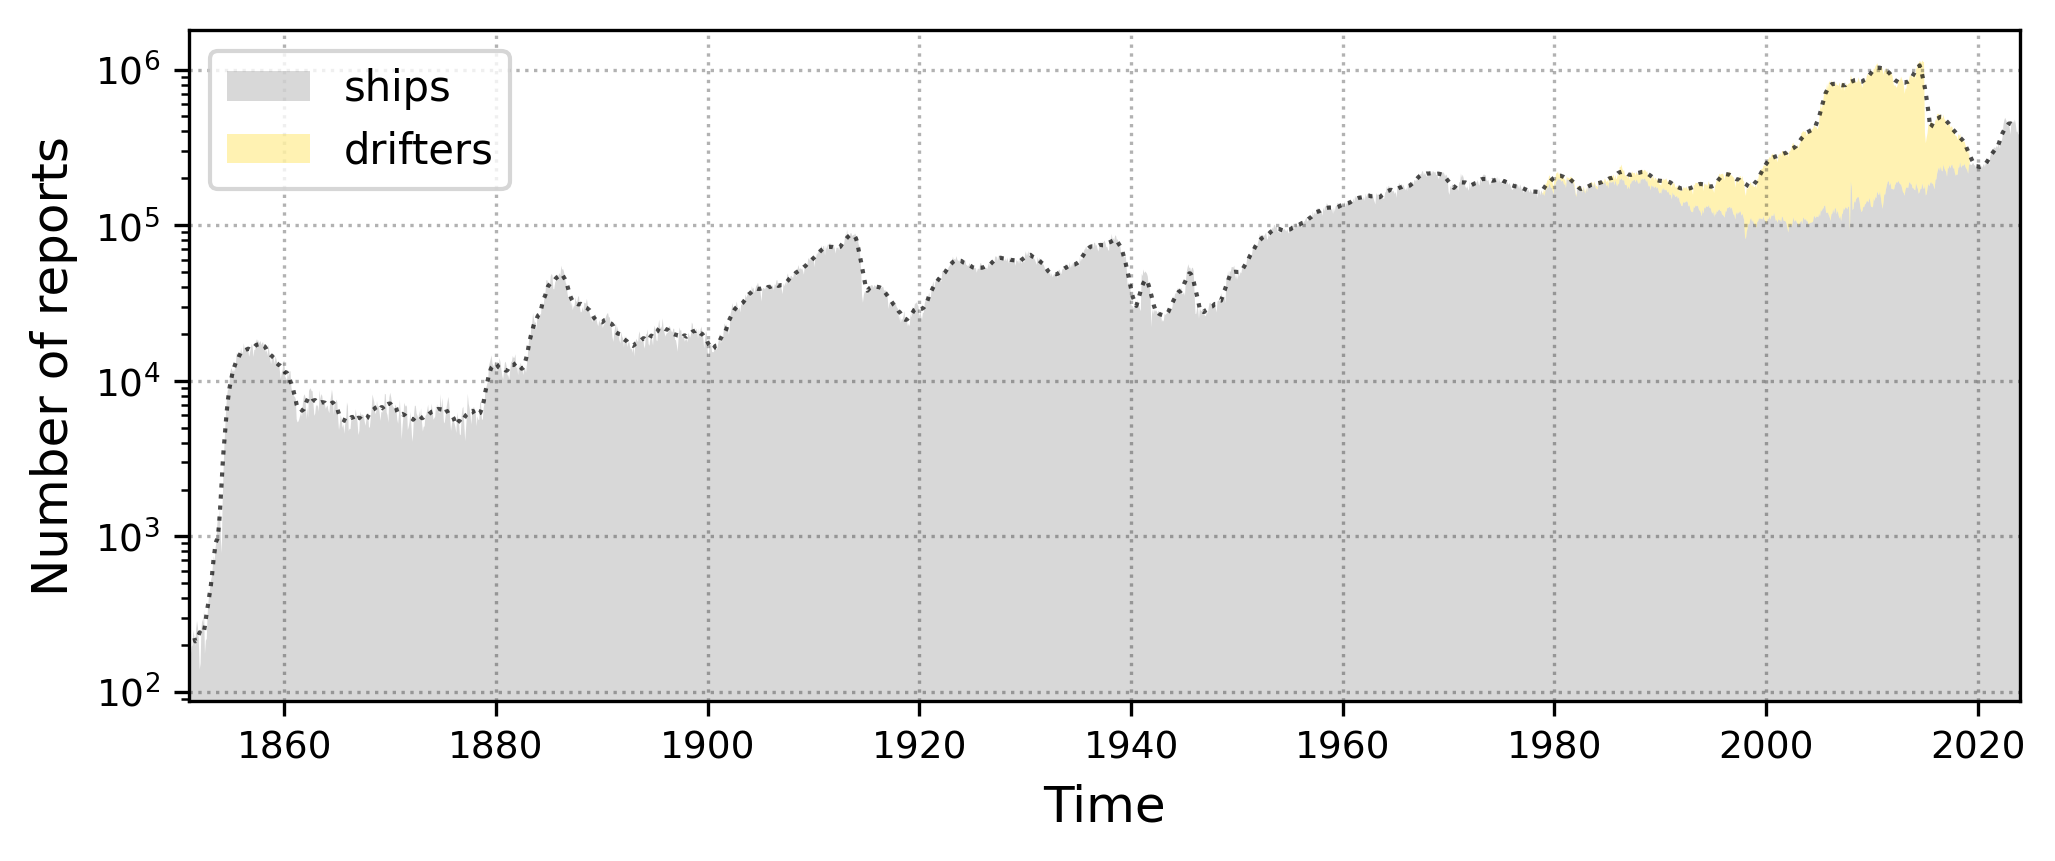
\includegraphics[width=0.8\textwidth]{resources/nreports-ts.png}
    \caption{Monthly number of marine in situ reports. The stacked areas indicate the monthly number of ship reports (grey) and drifting buoy reports (yellow). Only reports that have passed all the quality control checks are included. Time series have been smoothed using a 12-month running mean filter. Note the logarithmic scale in the y axis.\\}
    \label{fig:nreports-ts}
\end{figure}

\begin{figure} [h]
    \centering
    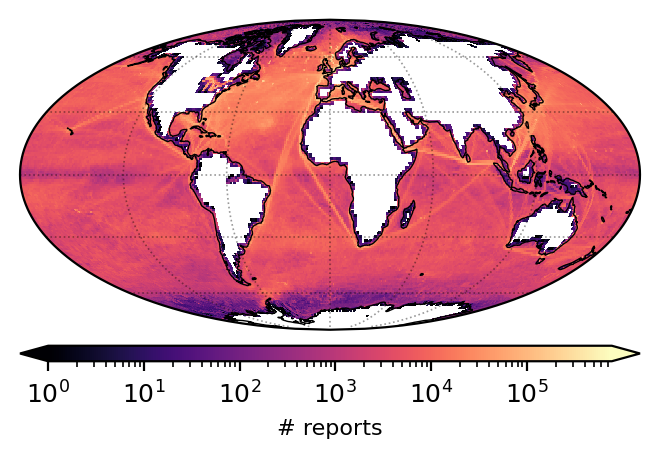
\includegraphics{resources/header-reports-map-optimal.png}
    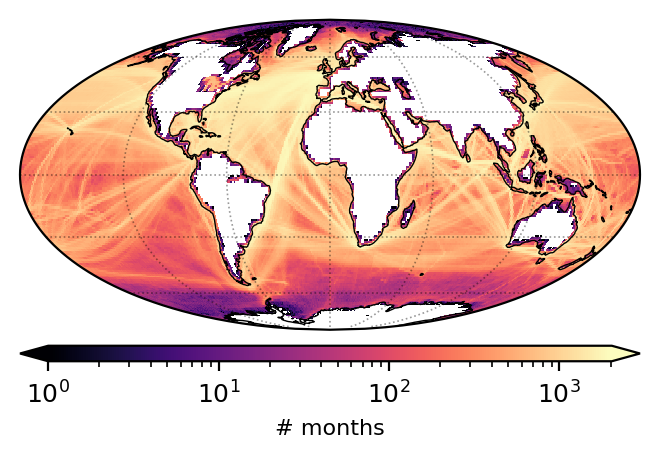
\includegraphics{resources/header-months-map-optimal.png}
    \caption{Spatio-temporal distribution of marine data holdings \datatimerange{}. Left: number of reports per grid cell; right: number of months with at least 1 report. Grid size is 1x1. Note logarithmic colour scale. Only reports passing the report level QC checks flag have been included.\\}
    \label{fig:nreports-map}
\end{figure}

\begin{figure}
    \centering
    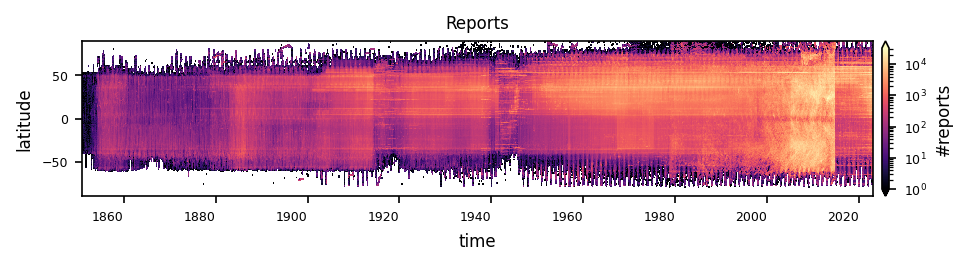
\includegraphics{resources/header-nreports_hovmoller_monthly}
    \caption{Spatio-temporal distribution of marine reports: latitude-time (Hovmøller) plots of number of reports. Data is binned and aggregated in 1° latitude × 1 month boxes. Only reports passing the report level QC checks have been included.\\}
    \label{fig:nreports-hovmoller}
\end{figure}

\FloatBarrier
\subsection{Metadata}
\subsubsection{WMO Publication Number 47 and other metadata}
WMO Publication No. 47 (https://www.ocean-ops.org/share/SOT/PUB47/), the International List of Selected, Supplementary and Auxiliary Ships, contains metadata on the ships, and observing methods used by those ships contributing to the WMO Voluntary Observing Ships Programme. 
A summary of the information available in WMO Publication No. 47 can be found in \cite{Kent2007}. 
This includes information on the ship dimensions and types, type(s) of instruments used, location of the sensors on board the ships and height of the sensors above the sea surface.  
A subset of the metadata from WMO Publication No. 47 has been included in ICOADS since Release 2.5 based on a basic match between the reports in ICOADS and the WMO Publication 47 edition coincident with the observation (\cite{Kent2007}, \cite{Woodruff2011}).

As part of C3S2 311 Lot 1 the WMO Publication 47 metadata has been reprocessed and selected fields, including ship names, types and instrument heights, have been included in this release. 
During the reprocessing duplicate records have been combined, reducing the number of records from around 875 000 to 255 000 over the period 1956 - 2020. 
Validity dates have been added, with the first record for a given ship extended by 1 year prior to its first appearance and the final record extended by 5 years. 
This allows for a period of time between a ship being recruited and it first appearing in WMO Publication No. 47 and a period where a ship continues reporting but is no longer registered by the original recruiting country. 
Limited quality control has been applied to the data, with correction of typographical errors and standardisation of entries. 
Similarly, heights have been corrected for known errors, such as incorrect packing of numeric data into alpha-numeric representation (e.g. i5 keyed instead of 15). 
In addition to WMO Publication No. 47, metadata is present in the ICOADS supplemental records for a small number of observations, including information such as ship type, barometer height, routes etc. 
%Where documentation exists this information has been decoded and included in this service.
Some information has been extracted from the ICOADS supplemental records and included in this service.

Figure \ref{fig:slp_heights} shows the fraction of ship observations passing quality control for which the sea level pressure observing height is known (red line). The blue shaded area indicates the 25th - 75th percentiles of the observing heights and the blue dashed line the median height. 
The earliest heights available are from the late 1870s for a period of \sim 15 years, with a significant proportion of the observations made during this period at a known height of around 5 m. 
There is then a large gap in the metadata until the 1960s where WMO Publication No. 47 becomes available and call signs begin to be used in the observational record allowing the metadata to be associated with the observations. 
However, the values before the 1970s should be used with caution, only a small fraction of the observations have been associated with the metadata, there is a large inter-quartile range and the median value is higher than expected.
This is likely due to a number of uncorrected heights in feet above sea level rather than meters above sea level but further work is required to fully understand the metadata.
Between 1970 and 2020 the median observation height increases from \sim 15 m to \sim 25 m.

The decrease in the proportion of observations with a known height from \sim 2014 is due to a decrease in the availability of call signs in the observational data due to call sign masking and use of generic call signs (such as SHIP) in response to security and commercial concerns of the participating Voluntary Observing Ships.
Metadata for the air temperature, humidity and wind speed observations does not become available until the 1960s although the observing heights are expected to be similar to that for pressure. 
From the 1970s onwards the change in heights (not shown) shows a similar trend to sea level pressure, with the temperature and humidity heights increasing from \sim 15~m to \sim 27~m. 
The increase in wind speed height is greater (not shown), increasing from \sim 15~m in the early 1970s to almost 35~m by 2020.

\begin{figure}[h]
    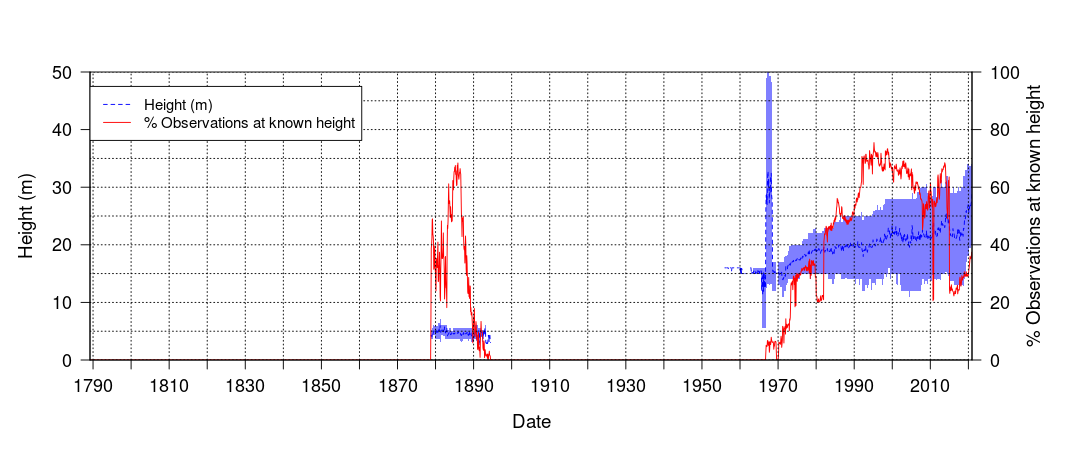
\includegraphics[width=18cm]{resources/brmh.png}
    \caption{Median sea level pressure observing height (blue) and \% of observations where the height is known (red). Also shown is the inter-quartile range of the observing height (blue shading).\\}
    \label{fig:slp_heights}
\end{figure}

\FloatBarrier
\subsection{Observing methods, coverage and known issues}
\subsubsection{Air temperature and humidity}
Figure \ref{fig:at-map} shows climatological values of the mean air temperature and dew point temperature over the period \datatimerange{}. 
Figure \ref{fig:at-nmonths-map} shows the number of months with at least 1 observation on a 1x1 grid. 
The clustering over the major shipping routes is clearly visible.
The air temperature and humidity measurements made on board ships have traditionally been made using liquid (mercury or alcohol) in glass thermometers (wet and dry bulb) sheltered from direct solar radiation, rain and sea spray and housed either in a fixed shelter or in a hand-held instrument. 
However, due to the need for the thermometers to be accessible the location of the thermometers is often not ideal, with the shelters sometimes located in poorly exposed locations and with inadequate ventilation.
This can lead to biases in humidity measurements due to inadequate ventilation of the wet bulb thermometers (e.g. \cite{Berry2011}; \cite{Willett2008}). 
Similarly, daytime air temperature measurements can contain biases due to the warming of the ship superstructure by solar radiation, in turn warming the air and giving biased air temperature measurements (\cite{Rayner2003}). 
Bias adjustments have been developed to account for these effects (e.g. \cite{Berry2004}) but have not been applied as part of this service. 
With the exception of the Second World War (e.g. see \cite{Cornes2020}; \cite{Kent2013NMAT}; \cite{Rayner2003}) pervasive biases have not been identified in the night time air temperature measurements or artificially ventilated wet bulb thermometers measurements during the period 1900 – 2020.
However, biases have been identified in the 19th Century and earlier data due to the use of thermometers located in the captains cabin (e.g. \cite{Chenoweth2000}).

% Figures for air temperature and humidity
\begin{figure}[h]
    \centering
    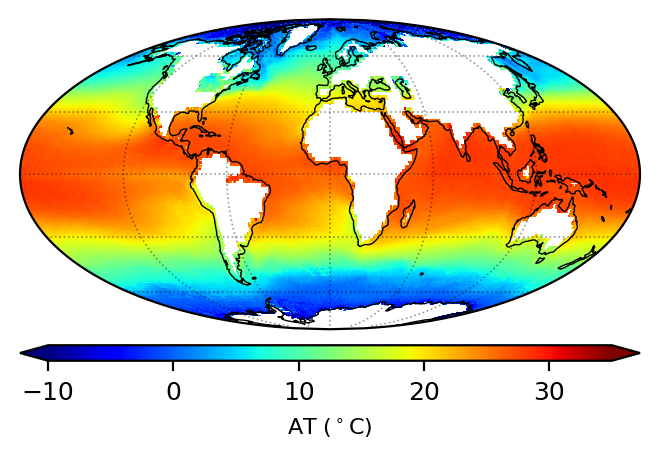
\includegraphics{resources/observations-at-mean-map-optimal.png}
    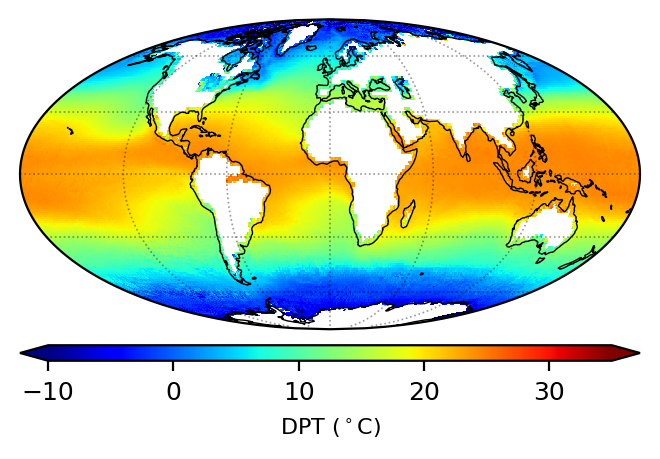
\includegraphics{resources/observations-dpt-mean-map-optimal.png}
    \caption{Mean air temperature (left) and dew point temperature (right) over the period \datatimerange{}. All observations passing quality control have been averaged to give monthly mean values. These have then been averaged to give the long term mean.\\}
    \label{fig:at-map}
\end{figure}
\FloatBarrier
Another factor that could lead to biases are systematic changes in the height at which the observations are made. The average observation height on merchant ship has has changed substantially over the period, ranging from \sim 4~-~5~m in the late 1800s, increasing to \sim 30~m in the late 2000s (Figure~\ref{fig:slp_heights}, \cite{Kent2007}, \cite{ Kent2013NMAT}). 
Adjustments to a fixed reference height are required to avoid inhomogeneities in the record and leading to underestimation of trends in the data. 
Adjustments are typically made based on Monin-Obukhov similarity theory and the approximation of a constant flux layer near the surface (e.g. \cite{Businger1971}). 
Observing heights are included with the observations where known but adjustments have not been made as part of this service.

\begin{figure}[h]
    \centering
    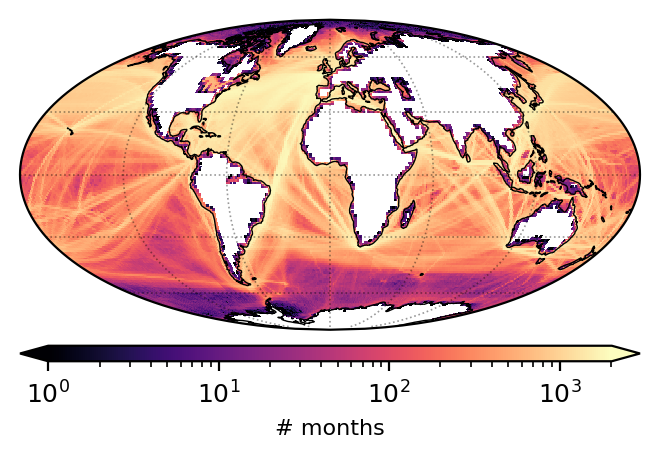
\includegraphics{resources/observations-at-months-map-optimal.png}
    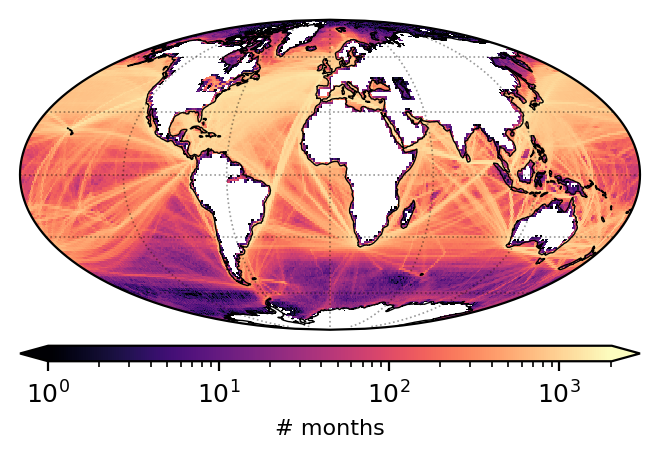
\includegraphics{resources/observations-dpt-months-map-optimal.png}
    \caption{Number of months with at least one observation of air temperature (left) or humidity (right) over the period \datatimerange{} on a 1x1 grid. Only observations passing quality control have been included.\\}
    \label{fig:at-nmonths-map}
\end{figure}

\FloatBarrier
\subsubsection{Sea surface temperature}
Figure \ref{fig:sst-map} shows climatological values of the mean sea surface temperature over the period \datatimerange{} (left) and the number of months with at least 1 observation on a 1x1 grid (right).
The clustering over the major shipping routes is clearly visible but with better sampling than before away from the shipping lanes due to the sampling by drifting buoys.
Sea surface temperature observations have been historically made using a wide variety of methods, ranging from wooden, canvas and rubber buckets to infrared radiometers. 
The most common methods are the bucket based and engine intake methods, both of which suffer from biases (\cite{Kent2017}). 
Due to evaporative and conductive cooling the water samples in the buckets can be biased low compared to the true sea surface temperature. 
Conversely, due to heat from the engine room, engine intake measurements can be biased warm. 
Bias adjustments have been developed and implemented when constructing gridded datasets from the observations (\cite{Kennedy2011_part2}). 
The quality of SST observations has been widely discussed (e.g. \cite{Kennedy2014}, \cite{Kent2017}).
As with the other parameters, no adjustments have been made to the observations to account for known biases as part of this service.

\begin{figure}[h]
    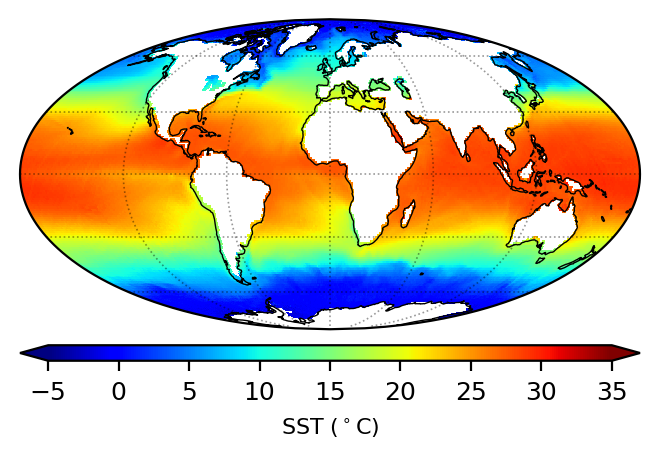
\includegraphics{resources/observations-sst-mean-map-optimal.png}
    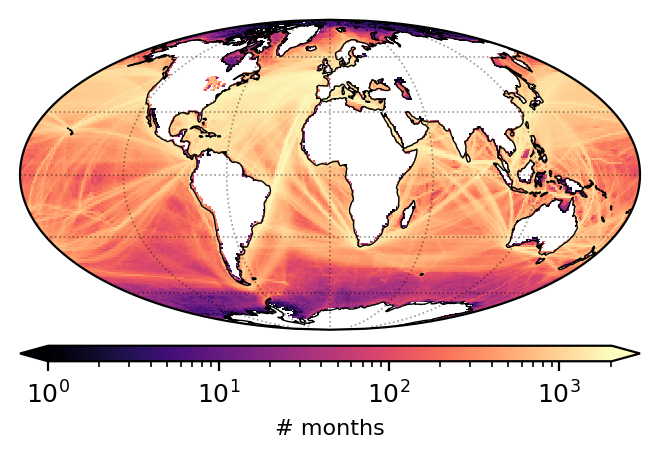
\includegraphics{resources/observations-sst-months-map-optimal.png}
    \caption{Mean sea surface temperature (left) and number of months with at least one observation (right) over the period \datatimerange{}. All observations passing quality control have been averaged to give monthly mean values. These have then been averaged to give the long term mean.\\}
    \label{fig:sst-map}
\end{figure}

\FloatBarrier
\subsubsection{Wind speed and direction}
Figure \ref{fig:wspd-map} shows climatological values of the mean wind speed and direction over the period \datatimerange{}. 
Figure \ref{fig:wspd-nmonths-map} shows the number of months with at least 1 observation on a 1x1 grid. 
As with the other parameters, the clustering over the major shipping routes is clearly visible. 
Wind speed observations made on board ships were historically made by estimating the wind force and recording the estimate using the Beaufort scale. 
This provides estimates of the upper, lower and mid-point wind speeds for each value on the scale at a reference height of 10 m. 
When Beaufort scale wind estimates have been converted to a speed the mid-point has typically been used. 
More recently, the visually estimated wind speeds have been estimated as a speed (e.g. knots or m/s) using the Beaufort scale as a guide. 

\begin{figure}[h]
    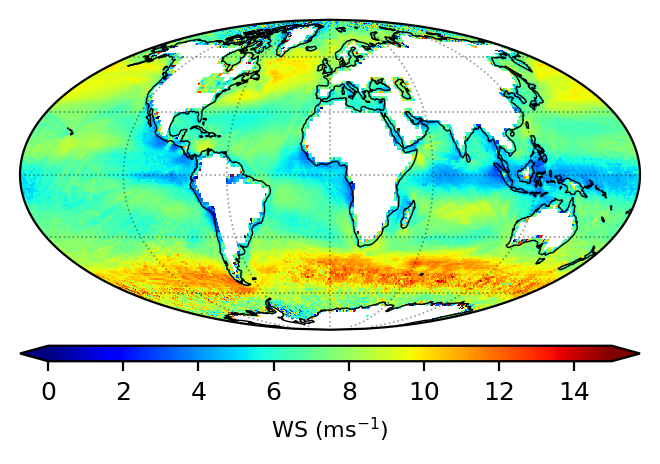
\includegraphics{resources/observations-ws-mean-map-optimal.png}
    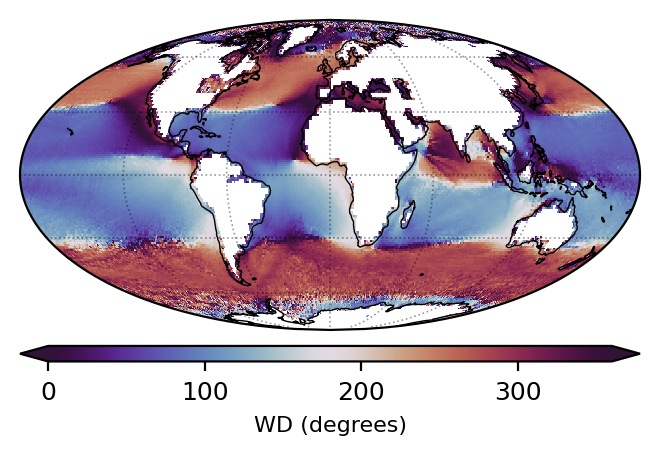
\includegraphics{resources/observations-wd-mean-map-optimal.png}
    \caption{Mean wind speed (left) and direction (right) over the period \datatimerange{}. All observations passing quality control have been averaged to give monthly mean values. These have then been averaged to give the long term mean.\\}
    \label{fig:wspd-map}
\end{figure}

Through comparison with instrumental measurements and co-located observations the original Beaufort scale has been shown to be biased and corrections proposed (\cite{Kent1997}).
Over the past several decades there has been an increasing move to using anemometers to observe and report the wind speed over the oceans. 
These measurements can contain biases due to the impact of flow distortion on the wind speed (\cite{Moat2005}).
As with the air temperature and humidity, the typical height of wind speed measurement has changed with time (e.g. \cite{Thomas2008}) and the measured values require adjustment to a common reference height.
Again, no adjustments have been made as part of this service.

\begin{figure}[h]
    \centering
    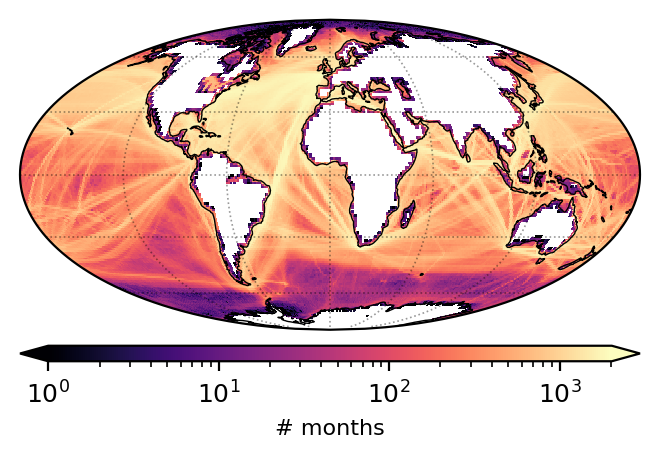
\includegraphics{resources/observations-ws-months-map-optimal.png}
    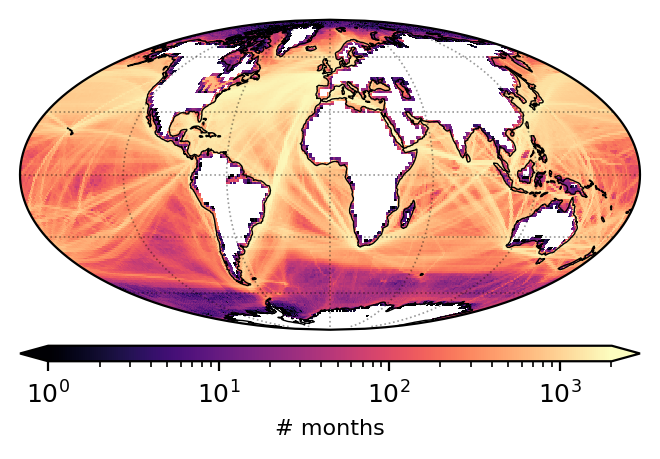
\includegraphics{resources/observations-wd-months-map-optimal.png}
    \caption{Number of months with at least one observation of wind speed (left) or wind direction (right) over the period \datatimerange{} on a 1x1 grid. Only observations passing quality control have been included.\\}
    \label{fig:wspd-nmonths-map}
\end{figure}

\FloatBarrier
\subsubsection{Sea level pressure}

Figure \ref{fig:slp-map} shows climatological values of the mean sea level pressure over the period \datatimerange{} (left) and the number of months with at least 1 observation on a 1x1 grid (right).
The clustering over the major shipping routes is clearly visible and, as with the sea surface temperature, better sampling away from the shipping lanes due to the sampling by drifting buoys can be seen.

Early pressure observations were typically made using mercury barometers, with a transition to marine aneroid barometers in the mid 20th century and to electronic instruments more recently. 
The different sensors each have corrections that need to be applied but these are typically applied either at the time of reporting or automatically prior to the values being read in the case of the electronic sensors. 
The mercury and aneroid barometers require correction for temperature and height above sea level, with an additional adjustment for gravity required for the mercury barometers. 
These corrections are believed to have been applied in the ICOADS data.
When looking at long term means / climatological values the observations also need to be corrected for diurnal and semi-diurnal oscillations (e.g. Ansell et al. 2006). These additional adjustments have not been applied as part of this service.



\begin{figure}[h]
    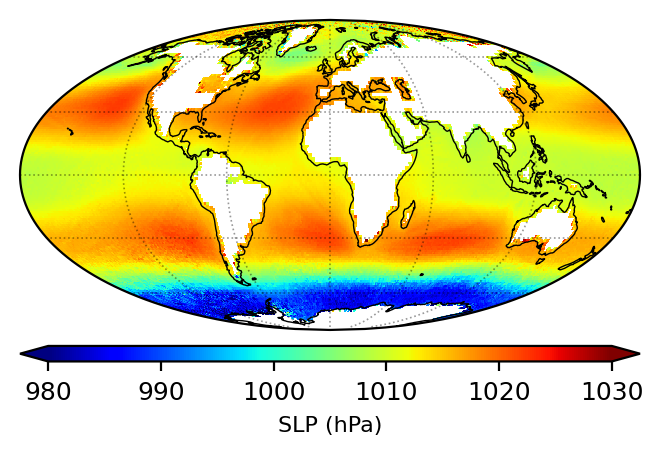
\includegraphics{resources/observations-slp-mean-map-optimal.png}
    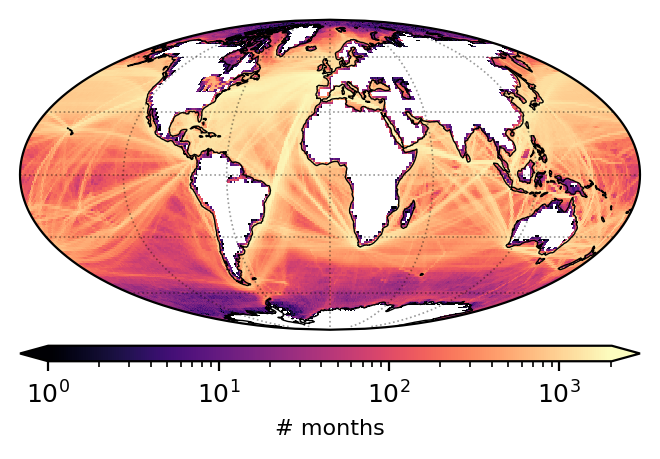
\includegraphics{resources/observations-slp-months-map-optimal.png}    
    \caption{Mean sea level pressure over the period \datatimerange{}. All observations passing quality control have been averaged to give monthly mean values. These have then been averaged to give the long term mean.\\}
    \label{fig:slp-map}
\end{figure}
\FloatBarrier
